\documentclass[aspectratio=169,xcolor=dvipsnames,UTF8]{beamer}
\usetheme{SimplePlus}

\usepackage{ctex}
\usepackage{CJK}
\usepackage{fontspec}
\usepackage{listings}
\usepackage{listings-ext}
\usepackage{color}
\usepackage{hyperref}
\usepackage{subfigure}
\usepackage{graphicx} % Allows including images
\usepackage{booktabs} % Allows the use of \toprule, \midrule and \bottomrule in tables
\usepackage{caption}
\usepackage{indentfirst}

% -- 压制警告
\PassOptionsToPackage{quiet}{xeCJK}

%图目录配置
\graphicspath{{images/}}
%图注解配置
%\captionsetup{font={tiny}}

% 配置参考文献
\usepackage[backend=biber,style=numeric,sorting=none]{biblatex}
\addbibresource{reference.bib} %BibTeX数据文件及位置
\setbeamerfont{footnote}{size=\tiny} %调整注脚的文字大小
%\setbeamertemplate{bibliography item}[text]

%----------------------------------------------------------------------------------------
%	标题页
%----------------------------------------------------------------------------------------

% 标题
\title[Web常见问题指北]{Web常见问题指北} 
\subtitle{浏览器同源策略及常见云产品涉及跨域问题和解决方法}

\author[Wei-Zhao] {Wei-Zhao}

\institute[Anchnet] 
{
    Anchen.Net
}
% 按编译日期计
\date{\today}


\begin{document}

%----------------------------------------------------------------------------------------
% 标题页
%----------------------------------------------------------------------------------------
\begin{frame}
    \titlepage
\end{frame}
%----------------------------------------------------------------------------------------


%----------------------------------------------------------------------------------------
% 目录页
%----------------------------------------------------------------------------------------
\begin{frame}{目录}
    \tableofcontents
\end{frame}
%----------------------------------------------------------------------------------------



%------------------------------------------------
\section{引言}
%------------------------------------------------
\begin{frame}{引言-跨域报错}
    \begin{figure}
          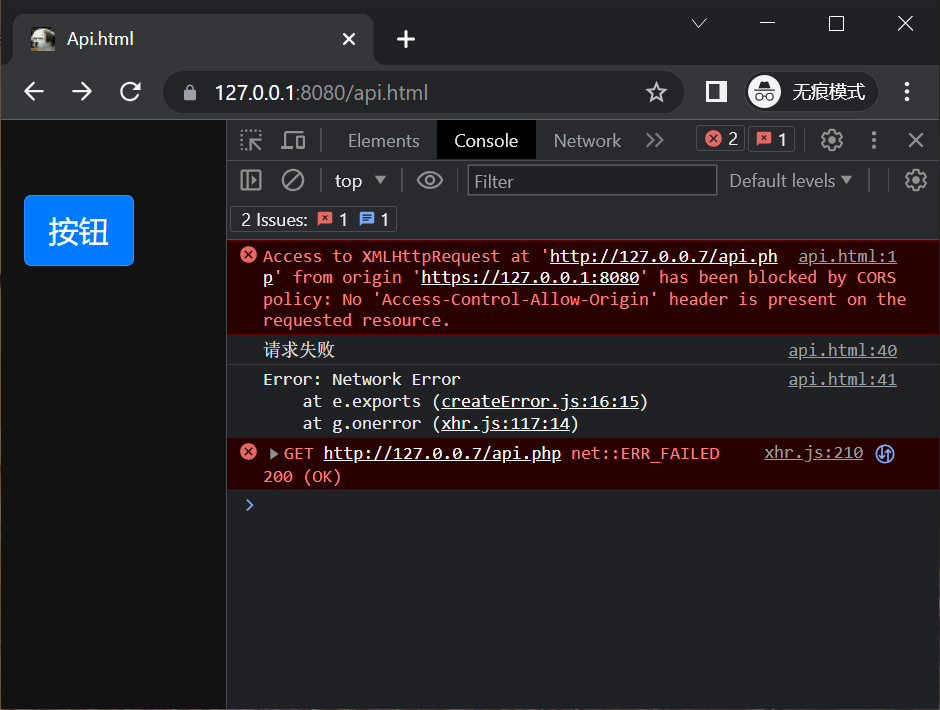
\includegraphics[width=0.48\linewidth]{cors-console-error.png.eps}
          %\caption{ \fontsize{0.5pt}{0pt} 1.1 Chrome控制台错误}
          %\begin{center}
          %	 1.1 Chrome控制台错误
          %\end{center}
          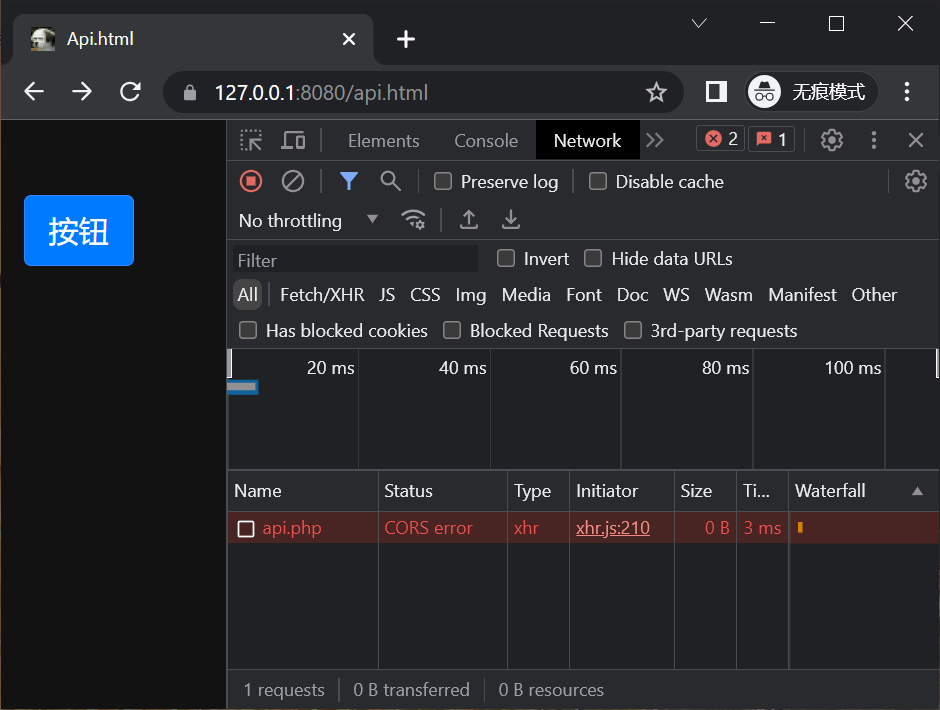
\includegraphics[width=0.48\linewidth]{cors-network-error.png.eps}
          %\caption{ \fontsize{0.5pt}{0pt} 1.2 Chrome控制台网络}
          %\begin{center}
          %	 1.2 Chrome控制台网络
          %\end{center}
    \end{figure}
%{\songti 宋体}	
%{\heiti 黑体}
%{\fangsong 仿宋}
%{\kaishu 楷书}
\end{frame}

%------------------------------------------------
\section{同源策略}
%------------------------------------------------
\begin{frame}{同源策略(Same Origin Policy)}
    \begin{block}{}
        \emph{浏览器的同源策略,限制了来自不同源的“document”或脚本,对当前“document”读取或设置某些属性。}
	\end{block}
	\vspace{2em}
    \setlength{\parindent}{2em}同源策略(Same Origin Policy)是一种约定,它是浏览器最核心也最基本的安全功能,如果缺少了同源策略,则浏览器的正常功能可能都会受到影响。可以说Web是构建在同源策略的基础之上的,浏览器只是针对同源策略的一种实现。
\end{frame}

\begin{frame}{存在跨域的情况}
    \begin{table}
        \begin{tabular}{l l c l}
            \toprule
            \textbf{当前页面URL}       & \textbf{被请求的URL}       & \textbf{是否跨域}       & \textbf{原因}       \\
            \midrule
                http://test.com/       & http://test.com/api/data       &       否 &       同源               \\
                http://test.com/       & https://test.com/api/data      &       是 &       协议不同(http/https)\\
                http://test.com/       & http://www.baidu.com           &       是 &       主域名不同           \\
                http://test.com/       & http://api.test.com/api/data   &       是 &       子域名不同           \\
                http://test.com:81/    & https://test.com:446/api/data  &       是 &       端口不同    \\
            \bottomrule
        \end{tabular}
        \caption{1-1 不同源明细\footfullcite{https://developer.mozilla.org/zh-CN/docs/Web/Security/Same-origin_policy}  } 
    \end{table}
\end{frame}

\begin{frame}{存在跨域的情况}
    \begin{table}
        \begin{tabular}{l l }
            \toprule
            \textbf{当前页面URL}       & \textbf{被请求的URL}        \\
            \midrule
            https://example.com/index.html &  http://vod.example.com/1.mp4     \\
            https://example.com/index.html &  http://example.com/1.mp4         \\
            \bottomrule
        \end{tabular}
        \caption{1-2 辨析}
    \end{table}
\end{frame}

%------------------------------------------------
\section{如何解决跨域报错}
%------------------------------------------------
\begin{frame}{如何解决跨域报错}
    \begin{enumerate}
        \item JSONP 
        \item CORS (跨域资源共享)
        \item Reverse Proxy (反向代理)
    \end{enumerate}
\end{frame}


\begin{frame}{JSONP方案-介绍}
JSONP的原理是利用不受浏览器同源策略限制的标签来发起请求。不受同源策略的标签有script、img、link(css)。后面两个标签无法回传数据,通常使用script加载js代码来回传数据。
\end{frame}

\begin{frame}{JSONP方案-交互时序}
    \begin{figure}
	\includegraphics[width=0.95\linewidth]{images/jsonp.eps}
        \caption{1-1 交互时序}
    \end{figure}
\end{frame}

\begin{frame}{JSONP方案-优缺点}
\begin{columns}[c]
	\column{.45\textwidth}
        \textbf{优点}
            \begin{enumerate}
                \item 兼容性高,能支持古老的浏览器
                \item 实现简单,即可轻松跨域
                \item 
               % \item 
            \end{enumerate}
        \column{.45\textwidth}
        \textbf{缺点}
            \begin{enumerate}
                \item 只支持GET请求
                \item 排错难度高,调用失败的时候不会返回HTTP状态码
                \item 安全性差容易被XXS攻击
            \end{enumerate}
\end{columns}
\end{frame}


\begin{frame}{CORS (跨域资源共享)-介绍}
CORS是通过给服务端设置
%   \begin{block}{}
%			\emph{查看演示}
%	\end{block} 
\end{frame}

\begin{frame}{CORS (跨域资源共享)-交互时序}
    \begin{block}{}
			\emph{查看演示}
	\end{block}  
\end{frame}

\begin{frame}{CORS (跨域资源共享)-优缺点}
    \begin{block}{}
			\emph{查看演示}
	\end{block} 
\end{frame}

\begin{frame}{ Reverse Proxy (反向代理)-介绍}
    \begin{block}{}
			\emph{查看演示}
	\end{block} 
\end{frame}

\begin{frame}{ Reverse Proxy (反向代理)-交互时序}
    \begin{block}{}
			\emph{查看演示}
	\end{block} 
\end{frame}

\begin{frame}{ Reverse Proxy (反向代理)-优缺点}
    \begin{block}{}
			\emph{查看演示}
	\end{block} 
\end{frame}

%----------------------------------------------------------------------------------------
% 参考文献页
%----------------------------------------------------------------------------------------
\begin{frame}{References}
    \footnotesize{
        \begin{thebibliography}{99}
        	\bibitem{article1}陈立辉,苏伟,蔡川,陈晓云.\emph{基于LaTeX的Web数学公式提取方法研究}[J], 计算机科学,2014(06)
  \bibitem{book1}William H, Press,Saul A. Teukolsky, William T. Vetterling, Brain P. Flannery, \emph{Numerical Recipes 3rd Edition: The Art of Scientific Computing} Cambridge Uninversity Press, New York, 2007.
  \bibitem{latexGuide}, Kopka Helmut, W.Daly Patrick,\emph{Guide to \LaTeX}, $4^{th}$ Edition. Available at \texttt{http://www.amazon.com}.
  \bibitem{latexMath} Graetzer George, \emph{Math Into \LaTeX},BirkhAuser Boston; 3 edition (June 22, 2000). 
        \end{thebibliography}
    }
    \printbibliography
\end{frame}

%----------------------------------------------------------------------------------------
% 结束页
%----------------------------------------------------------------------------------------

\begin{frame}
    \Huge{\centerline{\textbf{谢谢观看}}}
\end{frame}

%----------------------------------------------------------------------------------------
\end{document} 